\section{Information Hiding Algorithm}
\label{sec:scheme}

This section describes the encoding (hiding) and decoding (recovery) algorithms 
for our information hiding scheme and the rationale for them. 

\subsection{Overview}

Our scheme hides information in the program time of
individual bits of Flash. The program time is the time it takes 
for a bit to change from the erased state (1) to the programmed state (0).
Normally, a Flash memory controller performs a program operation
at a page granularity, and the latency of this program operation is
determined by the slowest bit in a page to be successfully written.
In order to determine the program time for each bit, 
which we refer to as {\em per-bit program time}, we use the partial
programming technique that is described in the previous section.

\begin{figure} 
\begin{center} 
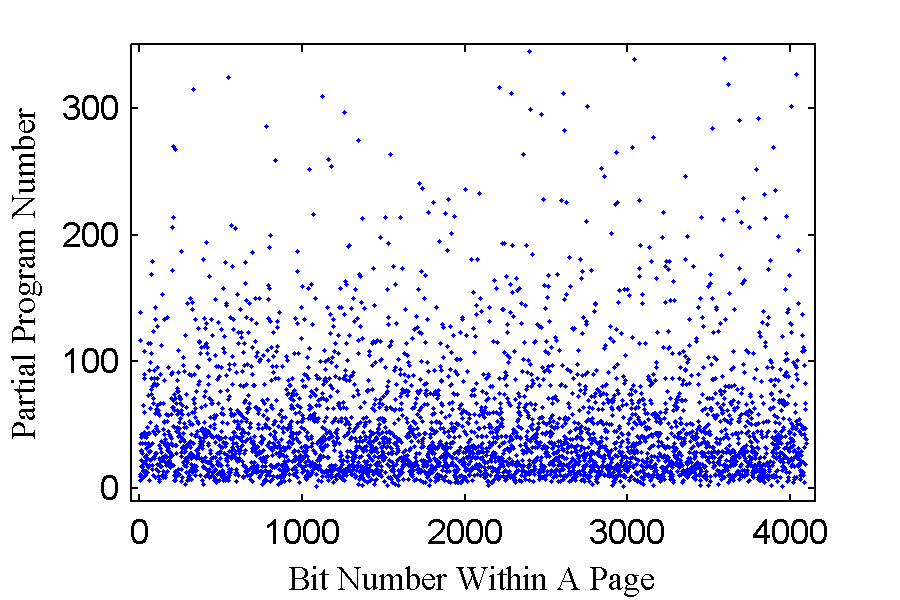
\includegraphics[width=\mywidth]{figs/program_numbers_c1_5e3pe_block1_page0.png} 
%\includegraphics[width=3.0in]{figs/eval_performance_diff_context.pdf} 
\caption{Raw partial program number for each bit in an example page.}
\vspace{-0.1in}
\label{fig:ptimeraw} 
\end{center} 
\end{figure} 

\begin{figure} 
\begin{center} 
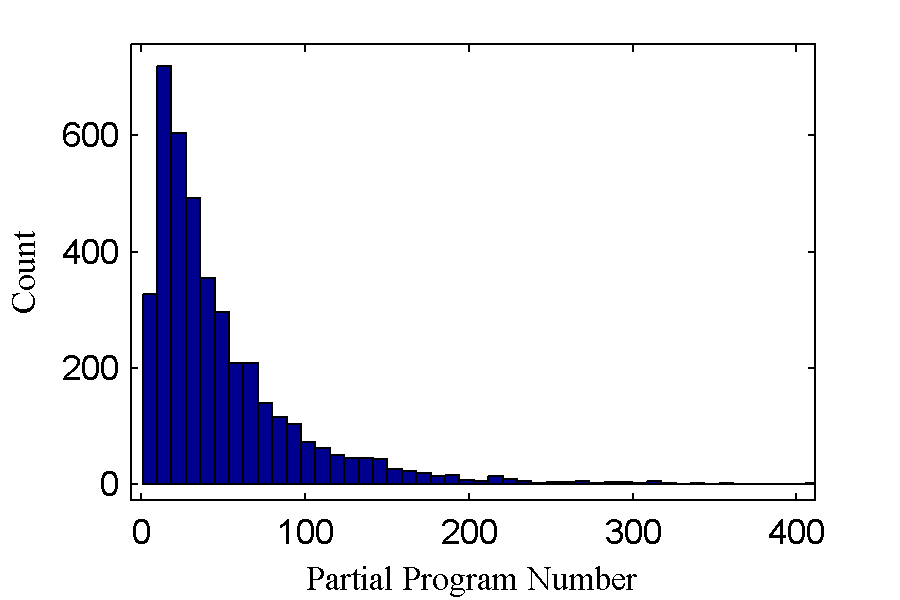
\includegraphics[width=\mywidth]{figs/hist_c1_block1_page1.png} 
%\includegraphics[width=3.0in]{figs/eval_performance_diff_context.pdf} 
\caption{Partial program time distribution for bits in a page.}
\vspace{-0.1in}
\label{fig:ptimehisto} 
\end{center} 
\end{figure} 

Figure~\ref{fig:ptimeraw} shows per-bit program times for a page. The plot
shows the number of partial program operations to flip state from 1 to 0 for each bit 
in a page. Because of process variations, the program time varies widely 
from bit to bit as shown in the figure. The per-bit program time distribution for the
page is shown in Figure~\ref{fig:ptimehisto}.
The wide distribution and noisy appearance of per-bit program times suggest that
small changes to each bit's program time would go unnoticed, and could be used to
carry a covert payload.

However, in order to hide information using the program time, we need to be able to 
intentionally change and control each bit's program time. Interestingly, in this
context, previous work has observed that program time tends to decrease as a Flash cell
becomes more worn-out \cite{grupp2009, trust2011}.
%varies depending on how worn-out a particular bit is
%A bit that is more worn-out shows a smaller program time.
In this work, we also found that how worn-out each bit is can be controlled
by selectively stressing a bit.
Although one can only program an entire page together, we can stress some bits
within a page more than others by controlling the value that we write.
During an erase operation, every bit
in a page is reset to an erased state (for example, assume that the erased state
represents '1').
On a program operation, only bits that switch to 0 experience
the program stress. When these bits are later erased, they also experience erase stress
as they are reverted to the 1 state. Therefore, bits that undergo
both switches (1 to 0 and 0 to 1) see the full program and erase stress
from one program and erase cycle. However, bits that store 1 will not be
switched to the 0 state by a program operation.
These bits see much less program and erase stress than their counterparts
which are programmed to 0 because their states do not need to change.
Therefore, by deciding whether to write a 1 or a 0 to each bit location 
in a page, we can control which bits are stressed more relative to 
other bits in the same page. 

In theory, if every bit had a similar program time without much variation,
we could hide one bit of information in every Flash bit by simply stressing or not
stressing the bit so that its program time encodes the hidden bit.
However, in practice, the program times of individual bits vary significantly
due to manufacturing variations, and intentional stress is often not sufficient 
to overcome the inherent variations; inherently slow bits will be likely to be
still slower than inherently fast bits even after being deliberately stressed.
To address this issue, we choose to encode 1 bit of hidden information %(stego-text)
using many bits in Flash memory. %(covertext). 
For each bit to hide, we choose a group of Flash bits and program them to the
same value, either 1 or 0. Effectively, this process encodes a bit in the collective
program time of the group. The averaging effect reduces variations among different
groups and allows the hidden bit to be more reliably recovered.

The use of a group also improves the security of the hiding scheme. In our scheme,
we use a key (hiding key) to select which Flash bits will be grouped together for
each hidden bit. If an attacker does not know the correct key, he or she cannot 
accurately identify which bits form a group together. 
Because an incorrect group is likely to contain both more stressed and less stressed
bits, the average program time of an incorrect group of bits will not show a clear
bias towards either 1 or 0. 

%Define "group" -- a group of bits in Flash that encode one bit of payload. This group
%is selected by a method known to the sender and receiver. We use a random selection
%of bits from the page to form a group.

\begin{figure} 
\begin{center} 
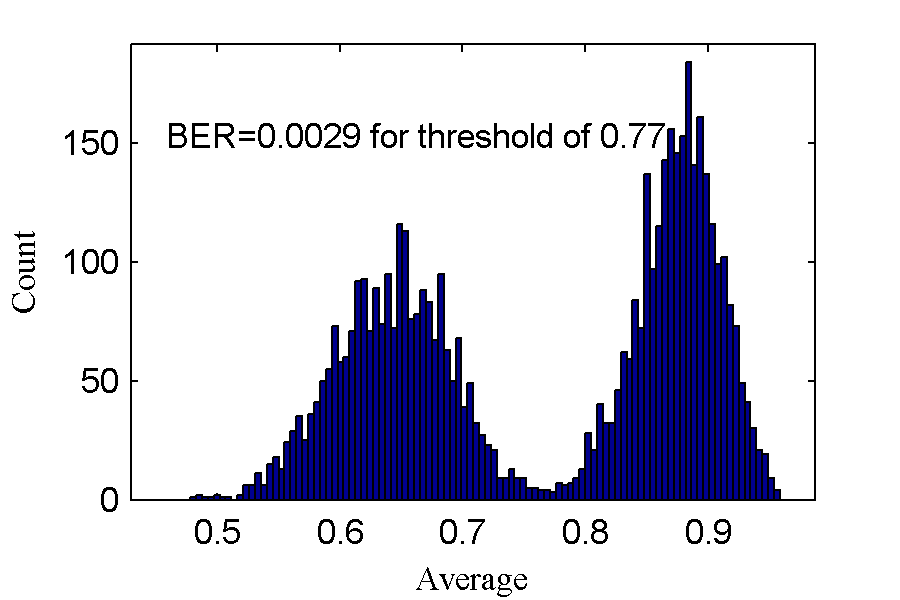
\includegraphics[width=\mywidth]{figs/5e3_histo_withkey.png} 
%\includegraphics[width=3.0in]{figs/eval_performance_diff_context.pdf} 
\caption{The distribution of the average program time of a group with a correct key.}
\label{fig:withkey_10blocks} 
\vspace{-0.1in}
\end{center} 
\end{figure} 

%To recover hidden information from the program time distribution,
%the intended recipient with the stego-key can compute the average
%program time for each group after the first thresholding. 
For example, Figure~\ref{fig:withkey_10blocks} shows the distribution of
the average program time of a correct group. In the experiment, we randomly selected
5,120 groups, each of which has 128 bits from a page, and hid either 1 or 0. 
As shown in the figure, these is an obvious gap in the distribution
between the fast and slow groups. Therefore, the value of hidden bits 
can be easily recovered through a simple thresholding. 
%We get a bit error rate (BER) of 0.0029 (0.29\%) in this case.
%even when a single
%quantization threshold ($X$) is used across all pages.


\begin{figure} 
\begin{center} 
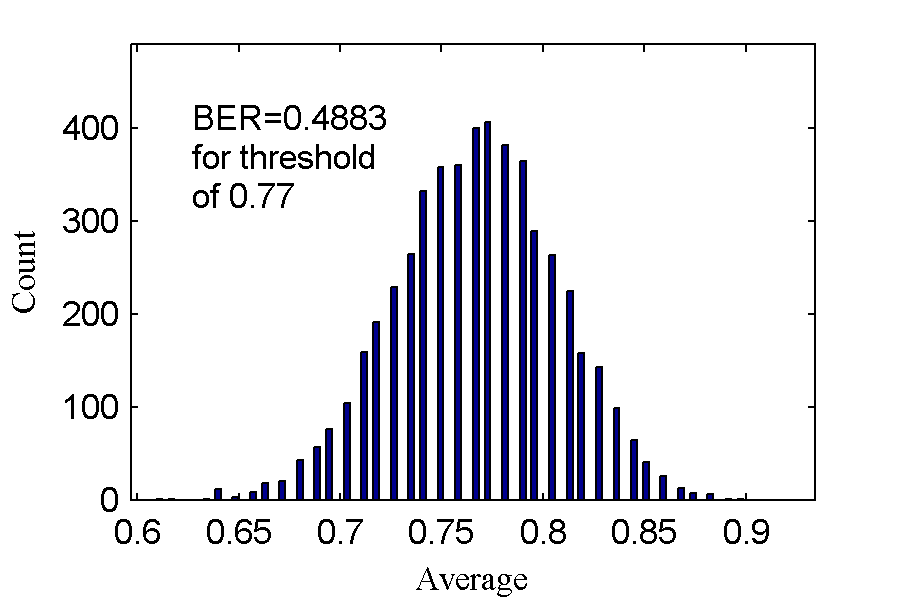
\includegraphics[width=\mywidth]{figs/5e3_histo_withoutkey.png} 
%\includegraphics[width=3.0in]{figs/eval_performance_diff_context.pdf} 
\caption{The distribution of the average program time of a incorrect group.}
\label{fig:withoutkey_10blocks} 
\vspace{-0.1in}
\end{center} 
\end{figure} 

On the other hand, Figure~\ref{fig:withoutkey_10blocks} shows the distribution
of the average program time when the hiding key is unknown. In this experiment,
we used a randomly selected hiding key. As shown in the figure, the average program
time of a group shows a normal distribution without any clear separation.
%The BER with the threshold $Th$ of 0.77 is 0.4883, which is close
%to 50\%. 
This result suggests that it is difficult for an adversary to recover hidden information 
without correct groupings because each group is likely to have both more and less
stressed bits.

%In fact, our experiments show that the distribution of individual bit's program
%time stays within a normal distribution even after the stress. As a result,
%it is difficult to tell whether any message is hidden within a page at all
%without knowing the correct key.



\subsection{Hiding Algorithm}

\begin{figure} 
\begin{center} 

%\begin{scriptsize}
\begin{center}

\begin{tabular}{|c|}
\hline
\begin{minipage}[t]{3.2in}



\begin{tabbing}
{\bf Algorithm I: Encoding }
\\
\\\emph{Part A -- Composing the message}
\\ 1 Fo\=r each selected page in a block
\\ 2 \>Generate the group for each message bit via the page hiding key
\\ 3 \>Assign each group 0 or 1 according to the embedded data
\\ 4 \>Fo\=r each bit
\\ 5 \>\>If\=\ its group will represent a message "1"
\\ 6 \>\>\>      Set it to be programmed 0
\\ 7 \>\>    Else
\\ 8 \>\>\>      Set it to be programmed 1
\\ 9 \>\>   End if
\\10 \>End for
\\11 End for
\\
\\\emph{Part B -- Writing the message to Flash}	
\\1 For each selected block
\\2 \>  For $i=1,2,..,N$ ($N$ is the number of Hiding PE cycles)
\\3 \>\>  Erase the block
\\4 \>\> Program every selected page
\\5 \>End for
\\6 End for


\end{tabbing}
\end{minipage}
\\ \hline
\end{tabular}
\end{center}
%\end{scriptsize}
 
\caption{An algorithm to encode (hide) a payload into Flash memory program time.}
\label{fig:encodingalg} 
\vspace{-0.25in}
\end{center} 
\end{figure}

Figure~\ref{fig:encodingalg} describes our methodology for hiding a payload in
program time of Flash memory. The algorithm is split into two parts: (A) composing the payload
by assigning bits of the message to groups of bits in Flash, and then (B) the actual process
of writing the payload to Flash by repeated program and erase stress.

For a given message, we first choose a set of pages and blocks in which to encode
the message based on the hiding key and the number bits that need to be hidden. 
Then, we divide the bits within each page into fixed size groups. % and record the groupings. 
Each group is used to store one message bit. 
The page, block, and group selections are based on the hiding key in a way that
cannot be predicted without the key. 
In our implementation, we used RC4 to choose the Flash bit locations for each message bit.

Then, the algorithm determines which value (0 or 1) needs to be written to each bit
location based on the message bit to be encoded.
If a group is to store a ``1'' value, we will
program (write a 0) the bits in the group, and the group will experience 
full program and erase stresses. If a group is to store a ``0'' value, the bits
in the group will be set to 1, and will see less stress.

With the payload mapped to bits in Flash memory, we perform the actual
write (program/erase) to Flash (Part B). We decide on a set number of stresses $N$ to exert
on the Flash. $N$ is chosen to ensure an acceptable
bit error rate without causing excessive stress. 
Each page is programmed $N$ times in order to imprint the
payload into the Flash.
In our experiments, we found that several hundred to a few thousand PE cycles are sufficient
for SLC chips. An even smaller amount of PE cycles are enough for MLC chips.


\subsection{Recovery Algorithm}

\begin{figure} 
\begin{center} 

\begin{footnotesize}
\begin{center}



\begin{tabular}{|c|}
\hline
\begin{minipage}[t]{3.2in}
\begin{tabbing}

{\bf Algorithm II: Decoding }
\\
\\\emph{Part A -- Reading the program time from Flash}
\\1 Fo\=r each selected block
\\2 \>Erase the block
\\3 \>Program every bit in the block to 0
\\4 \>Erase the block 
\\5 \>Fo\=r each selected page
\\6 \>\>Fo\=r $i=1,2, ..., M$  %(at least half of bits should flip after M iterations)
\\7 \>\>\>  Partial program the page to 0 (abort a program operation after time $T$)
\\8 \>\>\>  Read the page
\\9 \>\>\>  Fo\=r each bit in the page
\\10 \>\>\>\>If\=\ the bit changed from 1 to 0
\\11 \>\>\>\>\>   Set $program time$ for this bit to $i$
\\12 \>\>\>\>End if
\\13 \>\>\>End for
\\14 \>\>End for
\\15 \>\>Fo\=r each bit
\\16 \>\>\>If\=\ the bit did not flip
\\17 \>\>\>\>Set its $program time$ to be $M+1$ 
\\18 \>\>\>End if
\\19 \>\>End for
\\20 \>End for
\\21 \>Erase the block
\\22 End for
\\
\\\emph{Part B -- Extracting the payload message}
\\1 Fo\=r each selected block
\\2 \>Fo\=r each selected page
\\3 \>\>Calculate the median $X$ of the program times for all the bits
\\4 \>\>Fo\=r each bit
\\5 \>\>\>If its $programtime > (X/2)$
\\6 \>\>\>\>Set $program time$ to 1
\\7 \>\>\>Else
\\8 \>\>\>\>Set $program time$ to 0
\\9 \>\>\>End if
\\10 \>\>End for

\\11 \>\>Generate the group for each message bit with the page hiding key
\\12 \>\>For each group
\\13 \>\>\>Calculate the average program time for the group
\\14 \>\>\>If the average is less than $Th$
\\15 \>\>\>\>Recover the message bit: 1
\\16 \>\>\>Else
\\17 \>\>\>\>Recover the message bit: 0
\\18 \>\>\>End if
\\19 \>\>End for

%\\15 \>\>If the number of Hiding PE cycles $N < 2500$
%\\16 \>\>\>threshold $Th$ = fixed value $Th_f$
%\\17 \>\>Else
%\\18 \>\>\>sort the average program times
%\\19 \>\>\>find the maximum interval for the sorted program times
%\\20 \>\>\>threshold $Th$ = middle point of the maximum interval
%\\21 \>\>End if
%\\22 \>\>For each group
%\\28 \>\>End for

\\20 \>End for
\\21 End for
\end{tabbing}
\end{minipage}
\\ \hline
\end{tabular}
\end{center}
\end{footnotesize}
 
\caption{An algorithm to decode (recover) a payload from Flash memory program time.}
\label{fig:decodingalg} 
\vspace{-0.25in}
\end{center} 
\end{figure}


Figure~\ref{fig:decodingalg} describes our algorithm to decode a payload hidden 
by our encoding algorithm in Flash bit program time. Again, the algorithm is divided into
two parts: (A) physically reading the per-bit program time from Flash, and (B) recomposing
the payload from the program time distribution.

To read the hidden information, we must measure the program times for every bit in the pages
containing the hidden bits. To do so, we use the partial programming algorithm described 
in the previous section. We choose $M$ such that at the end of $M$ partial programs, 
more than half of the bits, are programmed.
% We used $M = 1200$ in our experiments. 
The program time of a bit is expressed as the number of partial program cycles needed to 
flip the bit from 1 to 0. 
For the bits that do not flip after the $M$ partial program operations, their program
times are set to be a constant above $M$ (i.e. $M+1$). 
%The length of a partial program
%($T$) is chosen to be small enough to be able to measure differences in program times.

To reconstruct the payload from the per-bit program times, we apply two thresholding steps. 
First, we compute the median program time $X$ across all bits within each page.
Then, the program time of each bit within a page is quantized based on the median;
if a bit's program time is above half the median
program time ($X/2$), then its program time is set to 1; otherwise it is set to 0.
%\textbf{TODO: HOW IS X/2 CHOSEN?}
($X/2$) was chosen empirically.

The bits are then divided into the groups specified by the hiding key. Within each group, 
the average of each individual bit's program times (now consisting of only 1 and 0) is 
computed, and the second thresholding step
is performed. Each bit in the payload is set to 1 if the average program time
of the corresponding group is below the threshold $Th$. Otherwise, the bit is set to 0.

In practice, with sufficient hiding PE cycles, we saw that there exists an obvious gap 
between the average program times of the more-stressed and less-stressed groups. 
As a result, it is straightforward to set the threshold $Th$ to distinguish the
two types of groups. For each page, we first sort the average program time of each
group. Suppose the sequence of sorted program times is $X0, X1, X2, ..., XN$. Then 
we calculate the intervals between the sorted average program times and get $X1-X0, X2-X1, ...$.
Suppose the maximum interval is $XM-XL$, then we set the threshold to be in the middle of that
interval; $Th = (XM+XL)/2$. In this way, we can get a per-page threshold. 
For the cases with low hiding PE cycles, where there is no clear gap between the two
clusters, the threshold is set to be a constant across pages based on the histogram
of the average program times from multiple blocks. 
 
%The threshold $Th$ is decided after plotting the averages. In practice,
%we saw that the groups would sort themselves into two clusters. Taking a histogram
%of the averages, we set the threshold $Th$ to be the lowest value in the gap between
%the two clusters.

For simplicity, we describe and evaluate the algorithm for the case where all bits 
within a selected page are used to hide bits. In order to make detection more
difficult, it is also possible to only use a small subset of bits within a page.
We leave this variant for future work.

